\scanpage{375}
\uuline{Calcul des $\operatorname{Ext}^i(G_a,G_a)$}

\uline{Prop} : Le $k[F]$-module $\operatorname{Ext}^i(G_a,G_a)$ (pour l'action de $\operatorname{Hom}(G_a,G_a)$ à droite) est de $F$ torsion $(i>\deleted{\unsure{0}}1)$.

\uline{Cor} : (\unsure{Milne|Mhre}) $G_a^\mathrm{perf}=$ restriction de $G_a$ au site parfait /$k$
\[
\begin{aligned}
G_a^\mathrm{perf}&=\lim_{\substack{\longleftarrow\\ F}}G_a\\
\operatorname{Ext}^i(G_a^\mathrm{perf},G_a^\mathrm{perf})&=0\qquad i>1.
\end{aligned}
\]
$\searrow$\quad\uline{Dém} : On considere la suite spectrale du coefficient universel
\[
\forall\ \text{fais simpl }X:\ E_2^{i,j}=\operatorname{Ext}^i_{\mathbb F_p}(\underline H_j(X),F)\Longrightarrow \mathbb H^{i+j}(X,F)
\]
En fait on va travailler dans la catégorie des fais de $\mathbb F_p$-modules

On travaille mod $F$ (au sens mod $\mathcal C$)
\[
\begin{aligned}
\operatorname{Hom}(G_a,G_a)&=k[F]\\
\operatorname{Ext}^1(G_a,G_a)&=0
\end{aligned}
\]
\margin{$\deleted{E^{*,j}}=\deleted{0}$\par $\deleted{j<n}$}

Dem par récurrence : On va considerer la s. spectrale précedente avec $X=K(G_a,n)$\qquad $\deleted{\operatorname{Ext}^i}$\quad $n$ grand.
\[
\begin{aligned}
E\qquad&\operatorname{Ext}^i(H_j(K(G_a,n)),G_a)\Longrightarrow H^*(K(G_a,n),G_a)\\
E_2^{i,n}&=\operatorname{Ext}^i(H_n(K(G_a,n)\ G_a)\\
&\underset{\operatorname{Ext}^i(G_a,G_a)}{\shortparallel}
\end{aligned}
\]
\figure{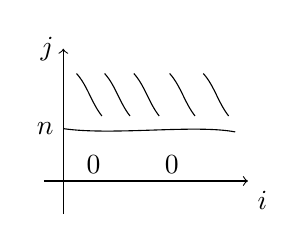
\begin{tikzpicture}[scale=.70]
\draw[->] (-.35,0)--(3.35,0) node[below right] {$i$};
\draw[->] (0,-.6)--(0,2.4) node[left] {$j$};
\draw (0,.95) node[left] {$n$}..controls (.9,.82) and (2.4,1.03)..(3.12,.89);
\node at (.55,.29) {$0$};\node at (1.97,.29) {$0$};
\foreach \x in {.24,.75,1.28,1.93,2.54}{\draw (\x,1.95)..controls (\x+.2,1.73) and (\x+.27,1.42)..(\x+.46,1.18);}
\end{tikzpicture}}
\[
\underline H_j(K(G_a,n)=\bigoplus G_a\qquad G_a\xrightarrow{p=0}G_a
\]
\mspage{377}
